\scanpage{49}
\mspage{\handwritten{17}}
\margin{\handwritten{\figure{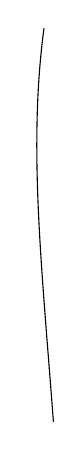
\begin{tikzpicture}\draw (0,0) .. controls (-.20,-1.5) and (-.03,-3) .. (.12,-5);\end{tikzpicture}}}}
\uline{Proposition} 11.\begin{tikzpicture}[x=1cm,y=1cm,baseline=(n.base)]\node (n) at (0,0) {11};\draw (-.15,.3)--(-.02,.3);\draw (-.07,-.08)--(-.07,-.25);\end{tikzpicture}. Le\deleted{t}\handwritten{t} \deleted{$k$ be a field}, $G$ be a \deleted{scheme in }group\deleted{s quasi-compact}\inserted{\handwritten{algebraic over the}} \deleted{over}\inserted{\handwritten{field}} $k$. The following conditions are equivalent:

(i) $G$ is affine.

(ii) $G$ is quasi-affine.

(iii) One can make $G$ act faithfully on a quasi-affine \inserted{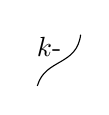
\begin{tikzpicture}[x=1cm,y=1cm,baseline=(n.base)]\node (n) at (0,0) {$k$-};\draw (-.15,-.5) .. controls (-.05,-.15) and (.35,-.25) .. (.4,.15);\end{tikzpicture}}scheme.

(iv) One can make $G$ act faithfully on a vec\deleted{o}\handwritten{t}or space over $k$ (not necessarily of finite \deleted{\unsure{t|d}}\inserted{d}imension).

(v) \deleted{(if $G$ is of finite type over $k$),} $G$ is isomorphic to a closed subgroup of a group $\mathrm{Gl}(n)_k$ .

\uline{Proof}. We have (i)$\handwritten{\Rightarrow}$(ii) trivially, and (ii)$\handwritten{\Rightarrow}$(iii), for $G$ acts faithfully on itself by left translations. We have (iii)$\handwritten{\Rightarrow}$(iv) for if $G$ acts \deleted{faithfully on $X$ quasi-affine over $k$, then it acts faithful-\linebreak ly on the affine envelope $X'=\operatorname{Spec}(\handwritten{\Gamma}($}\inserted{on $X$ quasi-compact and quasi-separated over $k$, it also acts} on the vector space $\handwritten{\Gamma}(X,\underline{O}_X)$, thanks to the fact that the formation of $f_{\handwritten{*}}(\underline{O}_X)$ ($f:X\handwritten{\to}\operatorname{Spec}k$ the structure morphism) commutes with every base change $S\handwritten{\to}\operatorname{Spec}k$ (EGA IV 1.7.12); thus it acts on the affine envelope $X'=\operatorname{Spec}(\handwritten{\Gamma}(X,\underline{O}_X))$, and the canonical morphism $X\handwritten{\to}X'$ is obviously compatible with the action of $G$; that said, if $X$ is quasi-affine i.e. $X\handwritten{\to}X'$ is an open immersion, and if $G$ acts faithfully on $X$, it acts faithfully on $X'$, or what amounts to the same thing, on the vector space $V=\handwritten{\Gamma}(X,\underline{O}_X)$, which proves the implication (iii)$\handwritten{\Rightarrow}$(iv).

\handwritten{S}uppose now \deleted{that $G$ is of finite type, and}\inserted{\handwritten{(iv), i.e.}} that $G$ acts faithful-\linebreak ly on the vector space $V$. Then\handwritten{,}by virtue of 11.10\handwritten{,}$V$ is an inductive limit of vector subs\handwritten{p}aces $V_i$ of finite di\handwritten{m}ension, stable under the action of $G$. If $K_i$ is the kernel of the induced action of $G$ on $V_i$ , i.e. of $G\handwritten{\to}\underline{\operatorname{Aut}}_{\inserted{\handwritten{V_i}}}\deleted{\unsure{(V_i)}}$, then $K_i$ is a closed subscheme of $G$, and the hypothesis that $G$ acts faithfully is at once expressed by the fact that \deleted{$K_{\unsure{1|i|l}}=e$ (grou} the intersection of the $K_i$ is the identity subgroup of $G$. Since $G$ is noethe-%
% archive sheet number: 48
